\documentclass[a4paper,10pt]{article}
\usepackage[top=0.75in, bottom=0.75in, left=0.55in, right=0.85in]{geometry}
\usepackage{graphicx}
\usepackage[latin1]{inputenc}
\usepackage{amsmath}
\usepackage{amsfonts}
\usepackage{amssymb}

\begin{document}

\begin{flushright}
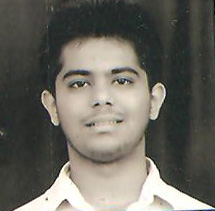
\includegraphics[width=3cm, height=4cm]{001.jpg}\\
\large
\textbf{\bigskip Ayush Bajaj}
\end{flushright}


\begin{flushleft}
	%contact information
	\textbf{\large Contact Information}:\\
	\hrule
	\bigskip
	\textbf{Adress:}            E-42 Dayanand Nagar\\
	\textbf{Contact:}   \texttt{9716989552}\\
	\textbf{Email:}             ayush95bajaj@gmail.com\\
	\bigskip
	\textbf{\large Career Objective} 
	\hrule
	\bigskip
	\textbf{To work in such a manner so that the ease of technology should benifit every common man}
	%education
	\textbf{\large  Education}:\\
	\hrule
	\bigskip
	\begin{tabular}{|c|c|c|c|c|}
   		\hline \textbf{ Degree}  & \textbf{College/school}  & \textbf{University} & \textbf{Passing Year} 			& 		\textbf{ Pass percentage} \\ 
   		\hline B.Tech Electronics & Maharaja Agrasen College  & Delhi University & 2017 & - \\ 
   		\hline 
			10+2 & Delhi Public School Ghaziabad & - & 2013 & 90 \\
    	\hline
\hline 
			10 & Delhi Public School Ghaziabad & - & 2011 & 10 CGPA \\
    	\hline
	\end{tabular} 
	\smallskip
		%projects

		\bigskip
    \textbf{Projects:}\\
    \hrule
	\smallskip
      \begin{enumerate}
      	\item  mine it bot(prototype model for detection of mines in form of boxes)
      	\item  Hand gesture controlled robot using xbee
      	\item  helio bot(prototype of capturing solar energy efficiently by movement of solar panel) 
      \end{enumerate}
	\end{flushleft}
	\end{document}
	